%%%%%%%%%%%%%%%%%%%%%%%%%%%%%%%%%%%%%%%%%%%%%%%%%%%%%%%%%%%%%%%%%%%%%%%%
%                                                                      %
%     File: Thesis_Introduction.tex                                    %
%     Tex Master: Thesis.tex                                           %
%                                                                      %
%     Author: Rui Santiago                         			   %
%     Last modified : 4 Junho 2015                      		   %
%                                                                      %
%%%%%%%%%%%%%%%%%%%%%%%%%%%%%%%%%%%%%%%%%%%%%%%%%%%%%%%%%%%%%%%%%%%%%%%%


\chapter{Trabalho anterior}
\label{chapter:Trabalho anterior}

%O sistema num chip em inglês System On Chip \acrlong{soc} é um chip integrado que tem integrado todas as funcionalidades de computador ou de um sistema electrónico, num único chip. Um \acrshort{soc} é constituído tipicamente por vários elementos interligados entre si por um barramento. Os elementos podem ser separados por grupos conformes os seus principais funcionalidades, os principais grupos são os seguintes: processamento, memoria, fontes de \textcolor[rgb]{1,0,0}{timing}, periféricos, interfaces externas, interfaces analógicas e gestores de energia. Na figura \ref{figures:ARM} pode se um exemplo de um diagrama de blocos de um \acrshort{soc}, onde se pode o barramento ligação dos elementos.
As { \it Coarse Grain Reconfigurable Arrays} (CGRAs) ganharam atenção nas duas últimas décadas \cite{Mei05,Lee00,Weinhardt03,Quax04,deSousa12}. As CGRAs são estruturas de hardware programável que podem ser construídas com conjuntos de processadores RISC ou apenas com componentes simples como ALUs, multiplicadores, shifters\cite{Tripp07,deSousa12}. As arquitecturas CGRA permitem normalmente reduzir o consumo de energia.
%\setlength{\parskip}{1 cm}
                  
O desenvolvimento de geradores de endereços capazes de suportar ciclos encadeados numa única configuração permitiu reduzir o tempo de reconfiguração das CGRAs\cite{deSutter10}. A ideia foi inspirada no uso de contadores em cascata para o gerador de endereços\cite{Carta06}. 
                         
Existem dois tipos de configuração: a configuração estática e a configuração dinâmica (reconfiguração). Na configuração estática o sistema é configurado uma única vez para correr um programa completo, o que é menos flexível\cite{Hartenstein01}. Na configuração dinâmica pode-se reconfigurar o sistema multiplas vezes durante um programa. No entanto, é necessário contabilizar o tempo de reconfiguração de modo que o desempenho seja satisfatório. 
                             
Existem dois tipos de sistemas reconfiguráveis: homogéneos e heterogéneos. No sistema homogéneo, todas as unidades de processamento são idênticas\cite{Ebeling96}, e permitem realizar um leque alargado de funções. No caso dos sistemas heterogéneos, cada unidade realiza uma tarefa específica\cite{Heysters03}. Apesar das redes homogéneas potêncialmente serem mais eficientes, as redes heterogéneas compensam com um rácio de uso de silício melhor e com uma melhor utilização energética\cite{Park12}. 
                          
Um compilador para este tipo de arquitecturas não pode usar apenas técnicas convencionais, mas também precisa de usar técnicas de colocação de componentes e encaminhamento de sinais ({\it Place and Route}), usadas também em FPGAs\cite{Betz99}.  
                          
%\vfill\newpage

\cleardoublepage
%\begin{figure}[!htb]
 % \centering
 % \includegraphics[width=0.5\textwidth]{Figures/ARM_SOC.png}
 % \caption[Diagrama de blocos de um soc ARM ]{Diagrama de blocos de um soc ARM }
 % \label{figures:ARM}
  %http://en.wikipedia.org/wiki/System_on_a_chip
%\end{figure}

%Os \acrshort{soc} têm uma vasta possibilidade de utilização desde um simples relógio até no mais avançado tecnologicamente como no desenvolvimentos de módulos para satélites, passando pela industria automóvel e com o aparecimento do arduino cada vez mais os \acrshort{soc} são utilizados em projetos de pequena escala desenvolvidos em casa, porque veio permitir a pessoas de com pouco ou nenhum conhecimento na área programar e efectuar debug no seu projecto com o \acrshort{soc}. A sua utilização traz vantagens com preço baixo, baixo consumo de energia e dimensões pequenas, como tudo o que existe também tem desvantagens sendo neste caso o baixo poder de calculo comparado com um computador. %http://www.extremetech.com/computing/126235-soc-vs-cpu-the-battle-for-the-future-of-computing

%Com uma área tão vasta de aplicações não é de estranhar que existam várias empresas \textcolor[rgb]{1,0,0}{a muito tempo} e varias startup no mercado a desenvolver \acrshort{soc} para fins totalmente distintos, cada empresa optimizando o seu para que foi desenvolvido.



% --------------------------------------------------------------------- 
%\section{Objectivos}
%\label{section:context}

%Uma startup no desenvolvimento de um projecto/produto necessita de um \acrshort{soc} para poder comercializar o seu produto. Na pesquisa do \acrshort{soc} ideal para o seu projecto encontram diferentes possibilidades, mas nenhuma preenchia todos os critérios pretendidos para o projecto. Como não foi encontrada uma solução ideal dos vários \acrshort{soc} disponíveis no mercado, a solução possível serias desenvolver o seu próprio \acrshort{soc} desenvolvido a medidas para o projecto.

% ----------------------------------------------------------------------
%\section{Motiva\c{c}\~ao}
%\label{section:motiva}

%\textcolor[rgb]{0,0,1}{desenvolver um sistema necessário para uma startup, o sistema vai ser desenvolvido a medida com o pretendido com a startup.}

%\section{Objectivos}
%\label{section:objectivo}

%A startup no desenvolvimento de um projeto/produto necessita de um \acrshort{soc}, como se pode ver na figura \ref{grafos:problema} que tem de ter a capacidade de processamento necessária para efetuar a descodificação e codificação de dados que irá receber e enviar. O \acrshort{soc} desenvolvido tem de permitir que sejas ligado mais dois modelos assíncronos permitindo a recolha de dados no local para posterior envio dos dados pelo modelo de comunicação. O produto é para ser usado em locais de difíceis acessos este terá de ter um baixo consumo, permitindo que a bateria funcione o maior tempo possível. Para alem do mencionado anteriormente também necessita de duas interfaces de comunicação \acrlong{uart} e \acrlong{gpio}. 

%\begin{figure}[!htb]
 % \centering
 % 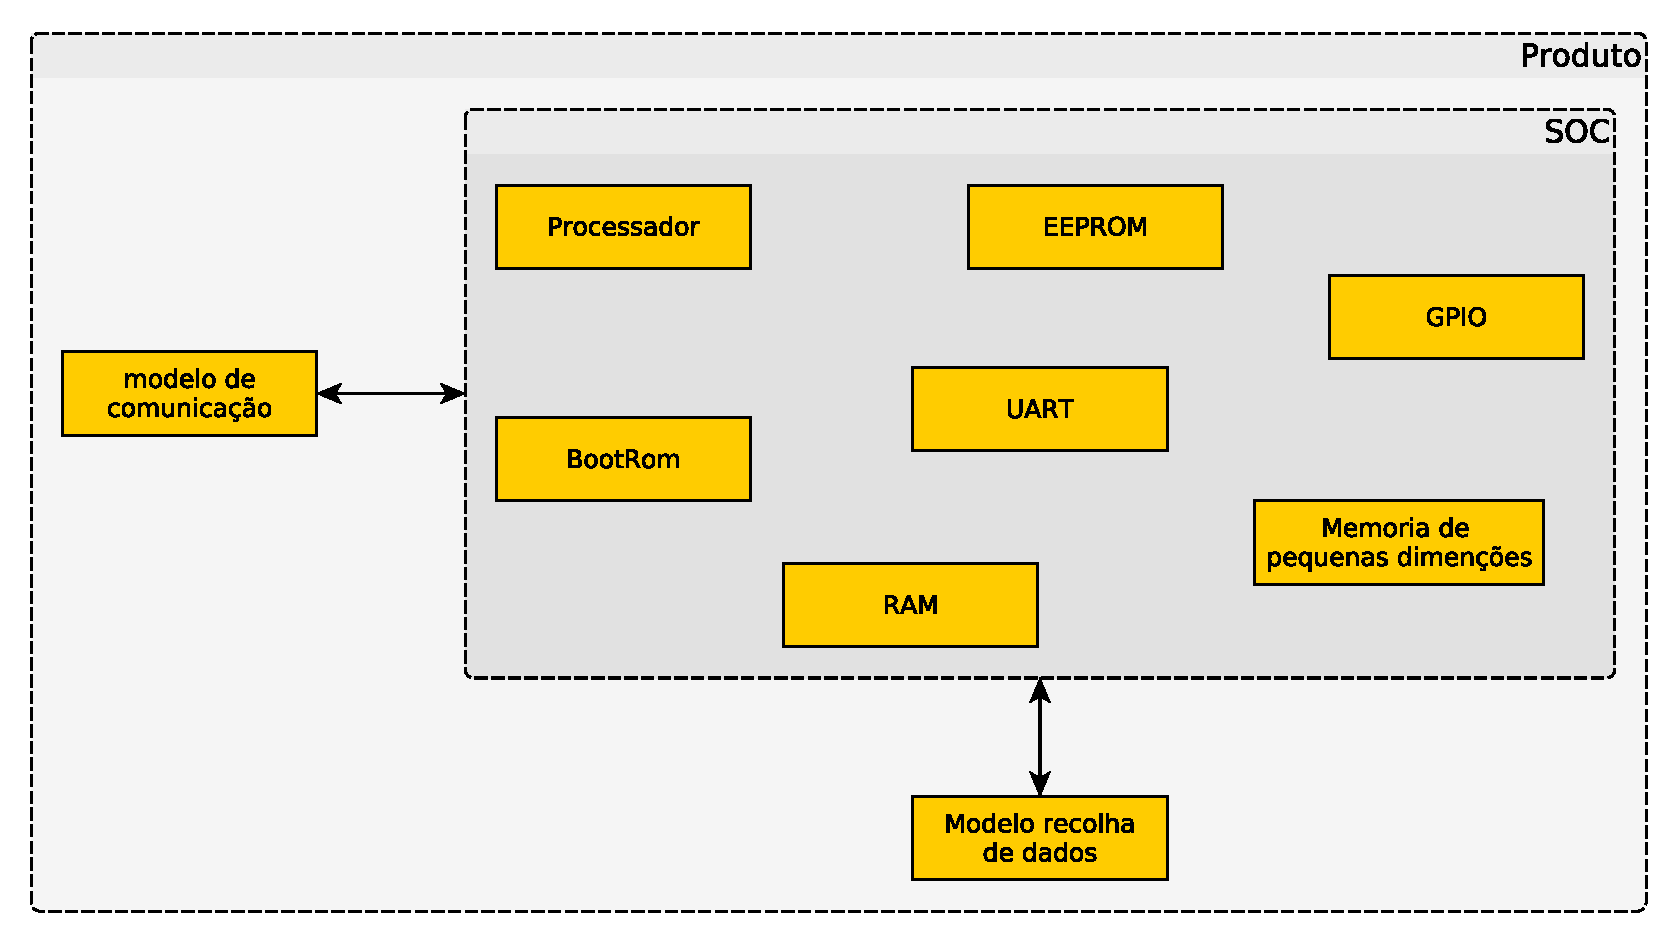
\includegraphics[width=0.5\textwidth]{grafos/problema.pdf}
 % \caption[SOC pretendido pela Startup]{SOC pretendido pela Startup}
 % \label{grafos:problema}
  %http://en.wikipedia.org/wiki/System_on_a_chip
%\end{figure}


%\section{Desafios}
%\label{section:desafio}


%Os principais desafios desta dissertação consiste no desenvolvimento de um sistema sintetizável que preencha todas as necessidades mencionadas pela startup.

%Desenvolver uma interface assíncrona necessária para a comunicação entre o \acrshort{soc} e os modelos de comunicação e de recolha de dados a ser desenvolvido pela startup.

%A criação de uma bootrom que carregua para a memoria principal o programa que se encontra na EEPROM. Ainda testa o mau funcionamento da EEPROM ou da memoria principal notificando o utilizador. 
